\subsection{Faster algorithm for \prob{IndependentSet}/$\shub$}
\label{section:indset-shub}

This section presents an algorithm for $\prob{IndependentSet}/\shub$. Specifically, we will prove that for every $\sigma \in \N$, there exists an $\varepsilon_{\sigma} > 0$, depending on $\sigma$, such that \prob{IndependentSet} can be solved in time $\O^\star((2-\varepsilon_{\sigma})^\ell)$, where $\ell$ is the size of a $\shub$ in the graph $G$. Unfortunately, the algorithm we developed is randomized and can only find the largest independent set of $G$ with high probability.

\medskip

\def\kl{\kappa^\text{large}}

Consider $\sigma \in \N$ to be reasonably large. For concretness, assume $\sigma \geq 10$ (since any $\shub[\leq 10]$ can be treated as a $\shub[10]$). Let $\delta \in \N$ be such that $\frac{1}{2}\cdot \frac{1}{10\sigma + 1}\cdot \frac{1}{2^\sigma}\cdot1.5^\delta \geq 1$ and let $\frac{1}{2} > \varepsilon > 0$ be such that $2^m - 1 \leq (2 - \varepsilon)^m$, where $m = \delta \cdot 2^\sigma$. We will first establish the following claim:

\begin{claim}
    \label{claim:random-algo-indset}
    There exists a polynomial-time randomized algorithm that, given a graph $G$ with a $\shub$ $X$ of size $|X| = \ell$, outputs an independent set $A$ of $G$ such that $$\Pr[A \text{ is a maximum independent set}] \geq \frac{1}{2}\cdot (2-\varepsilon)^{-\ell}.$$
\end{claim}

\begin{lemma}
    \label{lemma:random-algo-indset}
    There exists a randomized algorithm that, given a graph $G$, outputs an independent set of maximum size with probability $\geq \frac{1}{\sqrt{3}^n} \approx 1.73^{-n}$.
\end{lemma}

\begin{proof}
    If $G$ is edgeless, simply return the vertex set $V(G)$ as the maximum independent set. Otherwise, if $G$ contains an edge $\{u, v\}$, proceed as follows: randomly choose one of three options -- (1) include $u$ in the independent set, (2) include $v$, or (3) include neither $u$ or $v$.
    
    At each step, at least one of these choices is correct, and by making a choice, we effectively reduce the problem by removing two vertices from the graph. By induction, the probability of success after $\frac{n}{2}$ such steps is: $$\Pr[\text{success}] \geq \frac{1}{3}\cdot \frac{1}{3^{\frac{n-2}{2}}} = \frac{1}{3^{\frac{n}{2}}}.$$

    Thus, the success probability is approximately $1.73^{-n}$, as required.
\end{proof}

By definition, a $\shub$ $X$ of a graph $G$ ensures that $G - X$ consists of connected components, each with a size of at most $\sigma$. For any such component $A$, we consider the \emph{neighbourhood classes} of $A$ within $X$. A neighbourhood class of $A$ comprises all vertices in $X$ that have exactly the same neighbourhood in $A$. We denothe the set of neighbourhood classes of $A$ by $\kappa(A)$, or simply $\kappa$ when the context is clear. Observe that the number of neighbourhood classes $|\kappa|$ is bounded by $2^{|A|} \leq 2^\sigma$.

\medskip

For a subset $W \subseteq \kappa$, let $A^W = \{a \in A : N(a) \cap W = \emptyset\}$, where $N(a)$ denotes the neighbourhood of $A$. A class $B$ is called \emph{large} if $|B| > \delta$. We denote the set of all large classes in $\kappa$ by $\kl$. See \reffigure{fig:neighbourhood-classes} for a visual representation of these concepts.

\begin{figure}
    \centering
    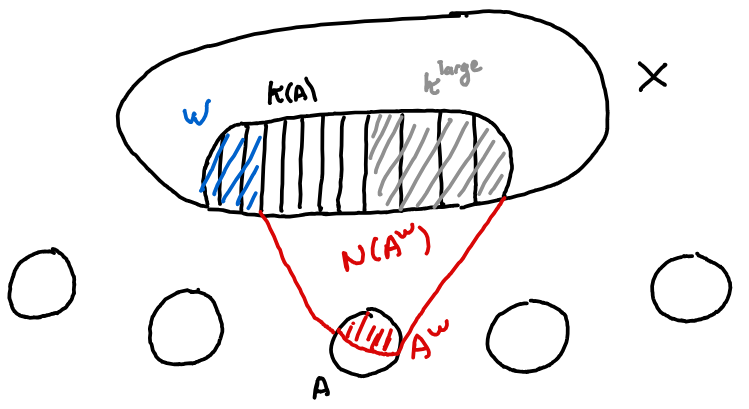
\includegraphics[width=.6\textwidth]{figures/neighbourhood-classes.png}
    \caption{}
    \label{fig:neighbourhood-classes}
\end{figure}

\medskip

Let $\alpha(G)$ denote the size of the largest independent set in a graph $G$. Note that for any subgraph $G'$ of $G$, $\alpha(G') \leq \alpha(G)$. Moreover, if $W_1 \subseteq W_2 \subseteq \kappa$, then $A^{W_2}$ is a subgraph of $A^{W_1}$.

\medskip

We categorize a component $A$ as follows:
\begin{itemize}
    \item \emph{trivial} if $\alpha(A^\emptyset) = \alpha(A^\kappa)$ (note that $A^\emptyset = A$),
    \item \emph{poor} if $\alpha(A^{\kl}) = \alpha(A^\kappa)$.
    \item \emph{rich} otherwise, i.e., if $\alpha(A^{\kl}) > \alpha(A^\kappa)$
\end{itemize}

\begin{observation}
    We can determine whether a component $A$ is trivial, poor, or rich in polynomial time.
\end{observation}

\begin{proof}
    Since $|A| \leq \sigma$, we can compute $\alpha(A')$ for any subgraph $A'$ of $A$ in constant time. 
\end{proof}

\begin{observation}
    If $A$ is trivial, we can remove $A$, run the algorithm on $G - A$, and then add $\alpha(A)$ to the result.
\end{observation}

\begin{proof}
    Since $A^\kappa$ is the subgraph of $A$ with no neighbours in $X$, and $A$ is trivial, we have $\alpha(A) = \alpha(A^\kappa)$. This means that the largest independent set $I$ of $G$ can always include $A^\kappa$ without affecting the selection of vertices in $I \cap (G - A)$. Thus, $A$ can be handled separately.
\end{proof}

From this point onward, we can assume there are no trivial components.

\medskip

Suppose $A$ is rich. We can compute the inclusion-wise minimal subset $W \subseteq \kappa(A) = \kappa$ such that:
\begin{itemize}
    \item $\kl \subseteq W$
    \item $\alpha(A^W) = \alpha(A^\kappa)$
\end{itemize}

Since $A$ is rich, $W \neq \kl$. This implies that $W - \kl \neq \emptyset$. Let $B \in W - \kl$. We define $M$ as followed: $$M \coloneqq B \cup \bigcup_{C \in \kappa - W} C \cup Z,$$ where $Z$ consists of one vertex from each class in $W - \{B\}$. See \reffigure{fig:construction-M} for a visual representation.

\begin{figure}
    \centering
    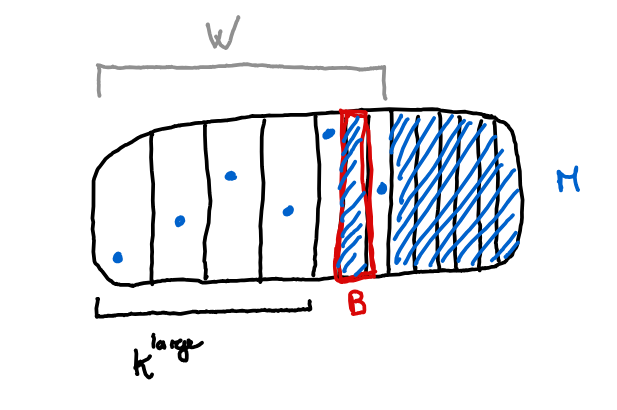
\includegraphics[width=.6\textwidth]{figures/construction-M.png}
    \caption{}
    \label{fig:construction-M}
\end{figure}

\begin{observation}
    $|M| \leq 2^\sigma \cdot \delta$
\end{observation}

\begin{proof}
    Every class included in $M$ consists of non large classes, which by definition, have a size at most $\delta$. Additionally, each class not directly included in $M$ contributes only one vertex to $M$. Since there are at most $2^\sigma$ classes, we obtain the bound $|M| \leq 2^\sigma \cdot \delta$.
\end{proof}

\begin{claim}
    There exists a maximum independent set $I$ such that $I \cap M$ is not of the form $Z \cup \{\text{one vertex $u$ from $B$}\}$
\end{claim}

\begin{proof}
    Let $I$ be a maximum independent set that has the smallest intersection with $X$. Suppose $I \cap M$ is of the form $Z \cup \{\text{one vertex $u$ from $B$}\}$. We will construct $I'$ as follows: $$I'\coloneqq I - \{u\} - (I \cap A) + \alpha(A^{W - \{B\}})$$

    \todo{change $\alpha(A^{W - \{B\}})$ in the formula above to be the set of size $\alpha(A^{W - \{B\}})$, not the number.} We know that $I \cap A \subseteq A^W$, since $I$ includes an element from every class in $W$ (the elements of $Z$ and $u$). Therefore, $\alpha(I \cap A) \leq \alpha(A^W)$. However, $\alpha(A^W) < \alpha(A^{W - \{B\}})$, because $W$ is inclusion-wise minimal such that $\alpha(A^W) = \alpha(A^\kappa)$, and $A$ is rich.

    The conclusion is that $|I'| \geq |I|$ but $|I' \cap X| < |I \cap X|$, which contradicts the hypothesis. Hence, $(I \cap M)$ cannot be of the form $Z \cup \{\text{one vertex $u$ from $B$}\}$. 
\end{proof}

Thus, we have an algorithm for handling rich components: we sample a pattern in $M$ from among the $2^{|M|} - 1$ possible options (since, as demonstrated in the previous claim, at least one pattern does not need to be considered). We assume this pattern and then recurse. By induction, assuming that we have an algorithm with a probability of success greater than $(2-\varepsilon)^{-\ell'}$ for a $\sdhub$ of size $\ell' < \ell$, we have:
\begin{align*}
    \Pr[\text{success}] &\geq (2^{|M|} - 1)^{-1}\cdot(2 - \varepsilon)^{-(\ell-|M|)}\\
    &\geq (2 - \varepsilon)^{-|M|}\cdot(2 - \varepsilon)^{-(\ell-|M|)}& \text{since $|M| \leq m = \delta \cdot 2^\sigma$ and by choice of $\varepsilon$ (see above)}\\
    &= (2 - \varepsilon)^{-\ell}
\end{align*}

From this point forward, we can consider that we are only dealing with poor components.

\medskip

Let us fix a maximum independent set $I$. We say that the component $A$ is \emph{underperforming} if $|I \cap A| = \alpha(A^{\kappa(A)}) < \alpha(A)$, since $A$ is not trivial.

\begin{observation}
    The number of underperforming components is at most $|X|$.
\end{observation}

\begin{proof}
    Suppose the number of underperforming components is greater than $|X|$. Then we can create another independent set $I'$ by choosing nothing from $X$ and, for each component $A$, selecting $\alpha(A)$ as $I \cap A$ (\todo{the set not the number}). This would give us:
    $$|I| = |I \cap X| + \sum_{A} |I \cap A| < |X| + \sum_{A} \alpha(A) - \underbrace{|X|}_{\text{due to the number of underperforming $A$}} = \sum_{A} \alpha(A) = |I'|$$

    This contradicts the assumptionthat $I$ is a maximum independent set. Therefore, the number of underperforming components cannot exceed $|X|$.
\end{proof}

We say that $I$ is \emph{restricted}, if the number of components that are not underperforming is at least $\frac{|X|}{10\sigma}$.

\begin{observation}
    If the number of components is at least $|X| + \frac{|X|}{10\sigma}$, then $I$ is restricted.
\end{observation}

\begin{proof}
    This follows directly from the fact that there are at most $|X|$ underperforming components.
\end{proof}

\subsubsection*{Final algorithm for poor components}

We now describe the final algorithm for handling poor components. If the number of components is $\geq |X| + \frac{|X|}{10\sigma}$, we assume that $I$ is restricted. If the number of components is $< |X| + \frac{|X|}{10\sigma}$, we toss a coin. Depending on the result, we assume $I$ is either restricted or not.

\medskip

If $I$ is assumed to be restricted: (1) sample a component $A$, (2) sample $B \in \kl(A)$: since $A$ is poor, $\kl(A)$ is non-empty (otherwise $A$ would be trivial), (3) assume $B \cap I = \emptyset$. Then recurse on $G - B$.

\begin{observation}
    If $A$ is not underperforming, then there exists a class $B \in \kl(A)$ such that $B \cap I = \emptyset$.
\end{observation}

\begin{proof}
    Since $A$ is not underperforming, $|A \cap I| > \alpha(A^\kappa)$. Given that $A$ is poor, we know $\alpha(A^{\kl}) = \alpha(A^\kappa)$. This implies there exists a vertex $u \in A \cap I$ such that $u \notin A^{\kl}$. By definition, $N(u) \cap \kl \neq \emptyset$, meaning there is at least one large class $B \in \kappa(A)$ where $I \cap B = \emptyset$.
\end{proof}

If $I$ is assumed not to be restricted: (1) sample a subset of components of size $\frac{|X|}{10\sigma}$, (2) assume that all other components are underperforming. This allows us to remove them and recurse on the remaining graph, which now has size at most $\sigma \cdot \frac{|X|}{10 \sigma} + |X| \leq \frac{11}{10}|X|$. We then apply \reflemma{lemma:random-algo-indset} to find the largest independent set of the remaining graph with probability $1.73^{-1.1|X|}$.

\subsubsection*{Probability of success}

\textbf{Case 1:} $I$ is restricted. The probability of success is given by:
\begin{align*}
    \Pr[\text{success}] &\geq \underbrace{\frac{1}{2}}_{\text{coin toss}} \cdot \underbrace{\frac{\frac{\ell}{10\sigma}}{\ell + \frac{\ell}{10\sigma}}}_{\text{proba to choose $A$ not underperforming}} \cdot \underbrace{2^{-\sigma}}_{\text{proba to choose the good class $B$}} \cdot \underbrace{(2 - \varepsilon)^{-\ell - \delta}}_{\text{induction, since $|B| > \delta$}}\\
    &\geq \frac{1}{2}\cdot \frac{1}{10\sigma + 1}\cdot\frac{1}{2^\sigma}\cdot 1.5^\delta \cdot (2 - \varepsilon)^{-\ell} & \text{$1.5^\delta$ since $\varepsilon \leq 1/2$}\\
    &\geq (2-\varepsilon)^{-\ell} & \text{by assumption (see above)}\\
\end{align*}

\textbf{Case 2:} $I$ is not restricted. The probability of success is given by:
$$\Pr[\text{success}] \geq \underbrace{\frac{1}{2}}_{\text{coin toss}} \cdot \binom{\ell + \frac{\ell}{10\sigma}}{\leq \frac{\ell}{10\sigma}}^{-1} \cdot \underbrace{1.73^{-1.1\ell}}_{\text{induction with \reflemma{lemma:random-algo-indset}}}$$
Here, the binomial factor is due to the fact that we need to choose the good not underperforming components among all the possible sets of components.

By assumption, since $\sigma \geq 10$, we have
$$\binom{\ell + \frac{\ell}{100}}{\leq \frac{\ell}{100}}^{-1} = \binom{1.01\ell}{\leq 0.01\ell} \leq 1.01^\ell \text{\todo{require verification}}$$

And finally, we have
$$\Pr[\text{success}] \geq \frac{1}{2}\cdot(1.01 \cdot 1.73^{1.1})^\ell \geq \frac{1}{2} \cdot (2 - \varepsilon)^\ell \text{\todo{require verification, do we have the same $\varepsilon$ has above?}}$$

This ends the proof of \refclaim{claim:random-algo-indset}.

\begin{theorem}
    For every $\sigma \in \N$, there exists an $\varepsilon > 0$ such that for any graph $G$ with a $\shub$ of size $\ell$, we can find the largest independent set of $G$ in time $\O^\star((2-\varepsilon)^\ell)$ with high probability.
\end{theorem}

\begin{proof}
    \todo{verification of this proof}
    
    We utilize the algorithm provided in \refclaim{claim:random-algo-indset}. By running this algorithm $(2-\varepsilon)^\ell$ times, the probability of successfully finding the largest independent set at least one is given by:

    $$\Pr[\text{success}] \geq 1 - (1 - \frac{1}{2}(2 - \varepsilon)^{-\ell})^{(2 - \varepsilon)^{\ell}}$$

    Since $(1 - a^{-1})^a$ quickly approaches $\frac{1}{e}$ as $a$ increases, this provides a constant probability of success. To further increase the probability of success, we can run the final algorithm a polynomial number of times, ensuring a success rate as high as desired.
\end{proof}